
\label{chap:experimental_results}


%FIXME: add text here

\subsection{Memory Synchronizer}

This section describes the various tests performed on the full/empty memory synchronizer used within the PDP firmware to synchronize data transitioning across clock domains. First, it discusses simulation results obtained through a full behavioral simulation of PDP. Secondly, it discusses using the memory synchronizer in a test setup and pitfalls that occurred with earlier implementations.

\subsubsection{Simulations}
Figure~\ref{fig:full_empty_sim} shows the simulated results of the full/empty memory synchronizer when transitioning to full and back to empty per clock cycle for writer and reader. For discussion about each signal and the expected internal behavior see chapter~\ref{sec:memorysync}. Each state transition in the simulation should look similar to the state transitions shown in Table~\ref{tbl:full_empty_circuit_states}.

\begin{figure}
    \centering
    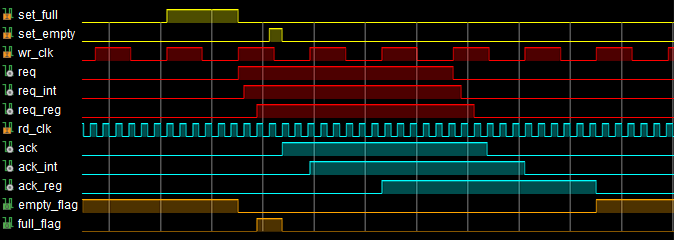
\includegraphics[width=1.0\textwidth]{fig/full_empty_sim.png}
    \caption{Full/Empty Circuit Simulation}
    \label{fig:full_empty_sim}
\end{figure}

The circuit holds a steady state until the {\it set full} signal is toggled for a single writer clock cycle. On the next writer clock cycle, the {\it req signal} transitions high and the {\it empty flag} transitions low. This transitions to the reader clock domain using the two flip-flop synchronizer scheme discussed in the implementation details. This transition starts in {\it req internal} which is metastable register used for the transition. The transition is fast because the reader clock is orders of magnitude faster than the writer clock. After this, the data transitions to {\it req reg} which is the output register in the reader clock domain. The full flag also transitions to high at this time. Once any corresponding buffer data is handled by the PDP firmware, the {\it set empty} signal is toggled for a single reader clock cycle. This causes the {\it ack} signal to transition high. This transitions to the writer clock domain using the two flip-flop synchronizer scheme. At the next rising edge of the writer clock this output is latched into {\it ack internal}. And a cycle later into {\it ack register} which is the output register in the writer clock domain.

Notice that the acknowledgement transitions take much longer to transition to the writer domain than request transitions take to transition to the reader domain. This is due to the slower writer clock. Once the {\it ack register} transitions, a single writer clock cycle later, {\it ack} transitions low. Subsequently, it transitions to the reader clock domain just as before, lowering much faster than the writer domain. Following this, the {\it ack} line is lowered and transitioned to the writer domain just as before. Then a cycle after the transition the {\it empty flag} transitions high, and the circuit is in the same state as it began. This follows the expected state transitions from Table~\ref{tbl:full_empty_circuit_states} with the only major difference being that the clock speed difference between the writer and reader results in differences in transition speed across clock domains.

The reader will note that these transitions take many cycles in practice due to the slow writer clock speed which may lead to undesired overflow behavior in some situations. In PDP, this is hidden by allocating enough internal buffers to allow for there to always be a buffer avaliable for a writer to fill. Additionally, the use of the two flip-flop synchronizer means that it takes more than a single reader clock cycle to transition data to the reader domain which could potentially have performance impacts in high speed operation for some use cases; however, given that an IRLED array's pixels charge much slower than a single reader clock cycle this doesn't pose a problem. Moreover, in practice, the {\it full flag} will transition in between two to three cycles of the reader clock depending on where the rising edge of the reader clock falls relative to the transitioning of the {\it req} signal.

\begin{figure}
    \centering
    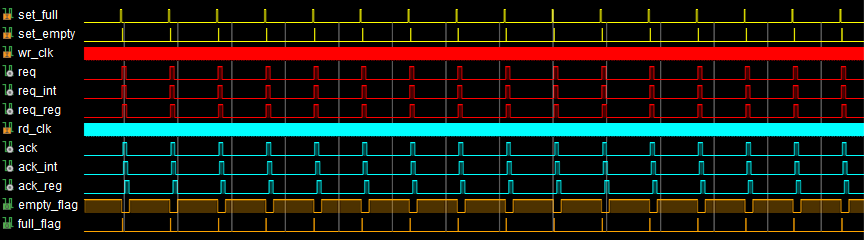
\includegraphics[width=1.0\textwidth]{fig/full_empty_row_sim.png}
    \caption{Full/Empty Circuit Full Row Simulation}
    \label{fig:full_empty_row_sim}
\end{figure}

\subsubsection{Verification}

\begin{figure}
    \centering
    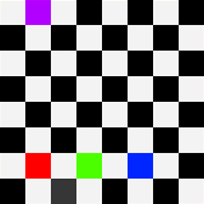
\includegraphics[width=0.25\textwidth]{fig/checker.png}
    \caption{Checker Input Image}
    \label{fig:checker_pattern}
\end{figure}

\begin{figure}
    \centering
    
\includegraphics[width=0.25\textwidth]{fig/random_noise.png}
    \caption{Random Noise Input Image}
    \label{fig:random_noise}
\end{figure}

\subsection{other stuff}
This section provides a few captures of simulation inputs and outputs to show how packets arrive and are processed by the architecture.

In Figure~\ref{fig:input_example} simulated HDMI is shown. When video data enable (write enable) transitions high words of data representing PDP packets start to stream in. These are indicated by Packet ID, X start, X end, Y start, Y end, and Packet Data. Each word would be stored in an SCB slot as indicated in the previous section. The final piece of data indicated is a reset packet. Note, that the data prior to Packet ID would be ignored as it does not represent a valid PDP command. It would be discarded by the valid controller.

\begin{figure}
    \centering
    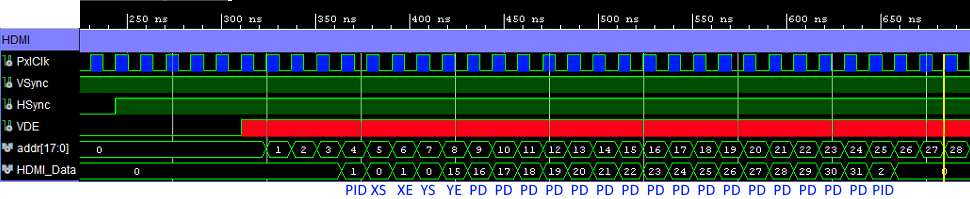
\includegraphics[width=1.0\textwidth]{fig/pdp_input_example.png}
    \caption{PDP Single HDMI Input Example Simulation}
    \label{fig:input_example}
\end{figure}

Figure~\ref{fig:output_example} shows the final output driven to the array. Highlighted in red is data from the write enable packet. Note, all values out are up shifted by 5 bits to be received by the DACs in the system. Additionally, the values are shown in reverse order from the input diagram. For example, 992 corresponds to the value of 31 on the input side. In purple the reset packet is shown with two stages of array writes. In the first stage, load line goes low. In the second stage the load line transitions high.

\begin{figure}
    \centering
    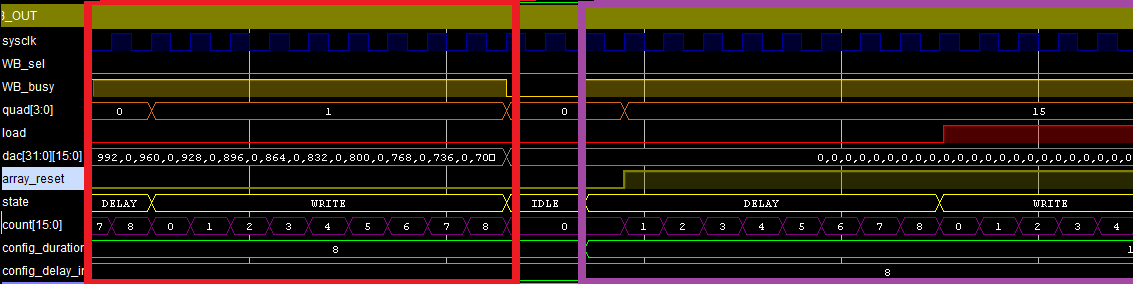
\includegraphics[width=1.0\textwidth]{fig/pdp_output_example.png}
    \caption{PDP Output Example Simulation}
    \label{fig:output_example}
\end{figure}
